%ps1.tex
%notes for the course Probability and Statistics COMS10011 
%taught at the University of Bristol
%2018_19 Conor Houghton conor.houghton@bristol.ac.uk

%To the extent possible under law, the author has dedicated all copyright 
%and related and neighboring rights to these notes to the public domain 
%worldwide. These notes are distributed without any warranty. 

\documentclass[11pt,a4paper]{scrartcl}
\typearea{12}
\usepackage{graphicx}
%\usepackage{pstricks}
\usepackage{listings}
\usepackage{color}
\lstset{language=C}
\usepackage{fancyhdr}
\pagestyle{fancy}
\lfoot{\texttt{github.com/COMS10011/2018\_19}}
\lhead{COMS10007 ps1 - Conor}
\begin{document}

\section*{Problem Sheet 1}

\begin{center}
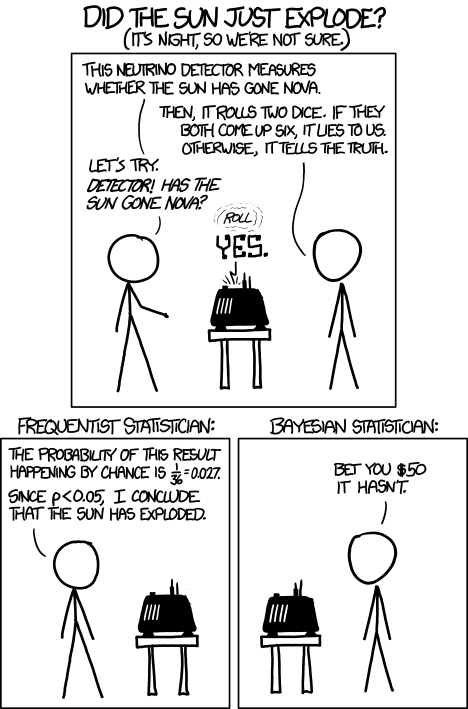
\includegraphics[width=7.5cm]{frequentists_vs_bayesians.png}
\end{center}

This is an xkcd cartoon that someone posted to the unit reddit, it is
\texttt{https://xkcd.com/1132/}.

\subsection*{Useful facts}

\begin{itemize}

\item \textbf{Combinations} The number of ways of choosing $r$ items out of $n$ is 
\begin{equation}
\left(\begin{array}{c}n\\r\end{array}\right)=\frac{n(n-1)(n-2)\ldots(n-r+1)}{r(r-1)(r-2)\ldots 1}=\frac{n!}{r!(n-r)!} 
\end{equation}

\item \textbf{Bayes's rule}
\begin{equation}
P(A|B)=\frac{P(B|A)P(A)}{P(B)}
\end{equation}

\item \textbf{Set notation}: If $C$ is a subset, the complement of $C$, that is the set of all the elements not in $C$, is written $\bar{C}$. For an event $C$, $\bar{C}$ is the event of $C$ not happening.
 
\item \textbf{Cards}: 52 cards made up of four suits; in each suit
  there are 13 values, ace, two through to ten and the jack, queen,
  kind.

\item \textbf{Poker hands}: the number of poker hands is 
\begin{equation}
\left(\begin{array}{c}52\\5\end{array}\right)= 2598960
\end{equation}

\end{itemize}

\newpage

\subsection*{Questions}

Four questions, each worth two marks with two marks for attendance.

\begin{enumerate}



\item In the poker hand two pair there are two pairs of cards with
  each card in the pair matched by value; the fifth card is a
  different value. What is the probability of two pairs when five
  cards are drawn randomly. In a full house there is one pair and one
  triple, what is the probability of getting a full house?

\item A student answers a multiple choice question with four options,
  one of which is correct. 80\% of students know the answer, 20\% of
  students guess and choose randomly. If a student gets the answer
  correct what is the chance they knew the answer.

\item In the xkcd cartoon above, what is the chance the Bayesian will
  when his or her bet if the chance the sun has exploded is one in a
  million? In reality the chance is, of course, much less than one in
  a million! Show the answer to six decimal places.

\item A three-sided dice is rolled three times. $X$ is the sum of the
  largest two values. Write down the probability distribution for $X$.

\end{enumerate}

\end{document}

